\documentclass{beamer}

\usepackage{Vor2018glærur}

\title{Tölvunarfræði 2}
\subtitle{Vika 6}

\begin{document}

\begin{frame}
	\titlepage
\end{frame}

\section{Inngangur}

\begin{frame}{Af hverju röðun?}
	\begin{itemize}
		\item Skoðum röðun í dag!
		      \begin{itemize}
			      \item Einföld röðunarreiknirit - kafli 2.1 í Algorithms
			      \item Sameiningarröðun - kafli 2.2 í Algorithms
		      \end{itemize}
		\item Röðun er vel leyst vandamál - af hverju skoðum við þetta svona vel?
		      \begin{itemize}
			      \item Röðunarreiknirit eru oft auðgreinanleg - góð æfing
			      \item Forritunarmynstur sem koma upp við röðun birtast oft í öðrum samhengjum
			      \item Röðunarreiknirit koma við sögu sem hluti af stærri reikniritum
		      \end{itemize}
	\end{itemize}
\end{frame}

\section{Comparable og uppbygging röðunarklasa}

\begin{frame}{Uppbygging röðunarklasa}
	\begin{itemize}
		\item Við munum forrita á móti Comparable skilunum
		      \begin{itemize}
			      \item Í stað þess að gera ráð fyrir að hluturinn sem unnið er með sé tilvik af ákveðnum klasa, þá gerum við ráð fyrir að hluturinn uppfylli ákveðin skil
			      \item Notum nafnið á skilunum eins og þau væru nafn á gagnagerð
			      \item Gerir röðunina sveigjanlegri án þess að láta eins og hún virki á hvaða klasa sem er
		      \end{itemize}
	\end{itemize}
\end{frame}

\begin{frame}{Uppbygging röðunarklasa}
	\javafile[firstline=10, lastline=23, fontsize=\scriptsize, label=SortTemplate.java]{Code/w6/SortTemplate.java}

	(Algorithms bls. 245)
\end{frame}

\begin{frame}{Hjálparaðferðir í röðunarklasa}
	\javafile[firstline=25, lastline=37, fontsize=\scriptsize, label=SortTemplate.java]{Code/w6/SortTemplate.java}

	(Algorithms bls. 245)
\end{frame}

\section{Eiginleikar röðunarreiknirita}

\begin{frame}{Eiginleikar röðunarreiknirita}
	\begin{itemize}
		\item Mörg mismunandi röðunarreiknirit eru til, getum metið þau m.t.t. mismunandi eiginleika
		      \begin{itemize}
			      \item Keyrslutími
			            \begin{itemize}
				            \item Teljum fjölda samanburða, víxlana (e. \emph{swaps}) og/eða fylkjaaðgerðir sem fall af inntaksstærð
			            \end{itemize}
			      \item Minniskrafa
			            \begin{itemize}
				            \item Þurfum við að geyma afrit af safninu sem við erum að raða?
			            \end{itemize}
			      \item Hversu almennt er það?
			            \begin{itemize}
				            \item Fyrstu röðunarreikniritin okkar virka á gögn sem uppfylla \texttt{Comparable}
				            \item Aðrir möguleikar eru til (sjá: Radix Sort, Counting Sort)
			            \end{itemize}
			      \item Er það stöðugt \eng{stable}?
		      \end{itemize}
	\end{itemize}
\end{frame}

\section{Nokkur röðunarreiknirit}

\begin{frame}{Valröðun}
	\begin{itemize}
		\item Valröðun \eng{selection sort} er einfaldasta röðunnarreikniritið okkar
		\item Lýsing:
		      \begin{enumerate}
			      \item Finnum minnsta stakið í safninu, setjum það fremst
			      \item Finnum næstminnsta stakið í safninu, setjum það næstfremst
			      \item Höldum áfram þar til safninu er raðað
		      \end{enumerate}
		\item Þarf $\sim \frac{n^2}{2}$ samanburði og $n$ víxlanir
		      \begin{itemize}
			      \item Margir samanburðir, lágmarksfjöldi víxlana
		      \end{itemize}
		\item Skoðum Selection.java
	\end{itemize}
\end{frame}

\begin{frame}[fragile]{Valröðun}
	\begin{minted}[frame=lines]{java}
int N = a.length;
for (int i = 0; i < N; i++) { 
    int min = i;
    for (int j = i + 1; j < N; j++)
        if (less(a[j], a[min])) min = j;
    exch(a, i, min);
}
    \end{minted}
	(Algorithms bls. 249)
\end{frame}

\begin{frame}[fragile]{Að sjá tannhjólin snúast}
	Getum notað \texttt{StdDraw} klasann úr algs4 til að teikna upp fylki
	\begin{columns}
		\column{0.6\textwidth}
		\javafile[firstline=12, lastline=19, gobble=8, fontsize=\scriptsize, linenos=false,label=StdDrawExample.java]{Code/w6/StdDrawExample.java}
		\column{0.4\textwidth}
		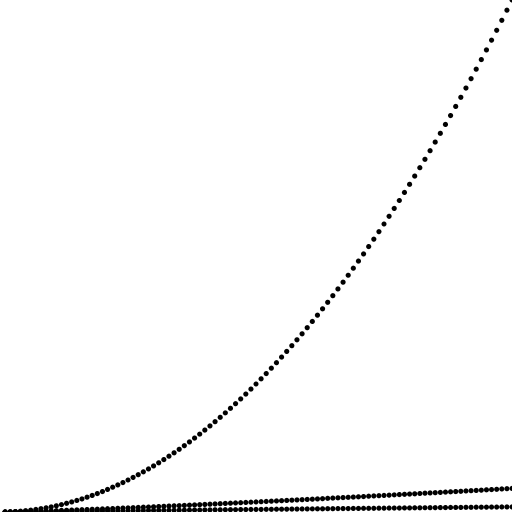
\includegraphics[width=\linewidth]{std-draw-example}
	\end{columns}
	Skoðum \texttt{SortVisualizer.java}
\end{frame}

\begin{frame}{Innsetningarröðun}
	\begin{itemize}
		\item Innsetningarröðun \eng{insertion sort} er aðferð sem er lík þeirri sem fólk notar venjulega við að raða raunverulegum hlutum
		\item Lýsing:
		      \begin{enumerate}
			      \item Höldum utan um ``raðaðan hluta'' til vinstri og ``óraðaðan hluta'' til hægri í safninu
			      \item Tökum það stak sem lengst er til vinstri í óraðaða hlutanum
			      \item Færum það lengra til vinstri þar til við rekumst á minna stak
			      \item Færum mörk undirsafnanna eitt stak til hægri og endurtökum
		      \end{enumerate}
		\item Mismunandi keyrslutími eftir tilvikum:
		      \begin{itemize}
			      \item $\sim \frac{n^2}{2}$ samanburðir og $\sim \frac{n^2}{2}$ víxlanir í versta tilvikinu
			      \item $\sim \frac{n^2}{4}$ samanburðir og $\sim \frac{n^2}{4}$ víxlanir ``að meðaltali''
			      \item $n-1$ samanburðir og engar víxlanir í besta tilvikinu
		      \end{itemize}
		\item Skoðum Insertion.java
	\end{itemize}
\end{frame}

\begin{frame}[fragile]{Innsetningarröðun}
	\begin{minted}[frame=lines]{java}
int n = a.length;
for (int i = 0; i < n; i++) {
    for (int j = i; j > 0 && less(a[j], a[j - 1]); j--) {
        exch(a, j, j - 1);
    }
    assert isSorted(a, 0, i);
}
assert isSorted(a);
    \end{minted}
	(Algorithms bls. 251)
\end{frame}

\begin{frame}{Sameiningarröðun}
	\begin{itemize}
		\item Sameiningarröðun \eng{merge sort} er skilvirk röðunaraðferð fyrir stóra lista
		\item Lýsing:
		      \begin{itemize}
			      \item Skilgreinum uppskiptingu á safninu svo úr verði hlutsafn
                  \item Skilgreinum uppskiptingar á sama hátt þar til hlutsöfnin eru af viðráðanlegri stærð
                  \begin{itemize}
                      \item Góð stærð: 1, þá þarf ekkert að raða
                  \end{itemize}
			      \item Sameinum hlutsöfnin svo úr verði raðað hlutsafn
		      \end{itemize}
		\item Þarf milli $\frac{n \log n}{2}$ og $n \log n$ samanburði, $\sim 6n\log n$ fylkjaaðgerðir
		      \begin{itemize}
			      \item Gott, en við þurfum auka minni!
		      \end{itemize}
		\item Skoðum Merge.java
		      \begin{itemize}
			      \item Hér er ofansækinni \eng{top-down} sameiningarröðun lýst
		      \end{itemize}
	\end{itemize}
\end{frame}

\begin{frame}[fragile]{Sameiningarröðun}
	\begin{minted}[frame=lines, fontsize=\scriptsize]{java}
private static void sort(Comparable[] a, Comparable[] aux, int lo, int hi) {
    if (hi <= lo) return;
    int mid = lo + (hi - lo) / 2;
    sort(a, aux, lo, mid);
    sort(a, aux, mid + 1, hi);
    merge(a, aux, lo, mid, hi);
}
public static void sort(Comparable[] a) {
    Comparable[] aux = new Comparable[a.length];
    sort(a, aux, 0, a.length - 1);
    assert isSorted(a);
}
    \end{minted}
	(Algorithms bls. 273)
\end{frame}

{
\usebackgroundtemplate{ \hspace{2cm}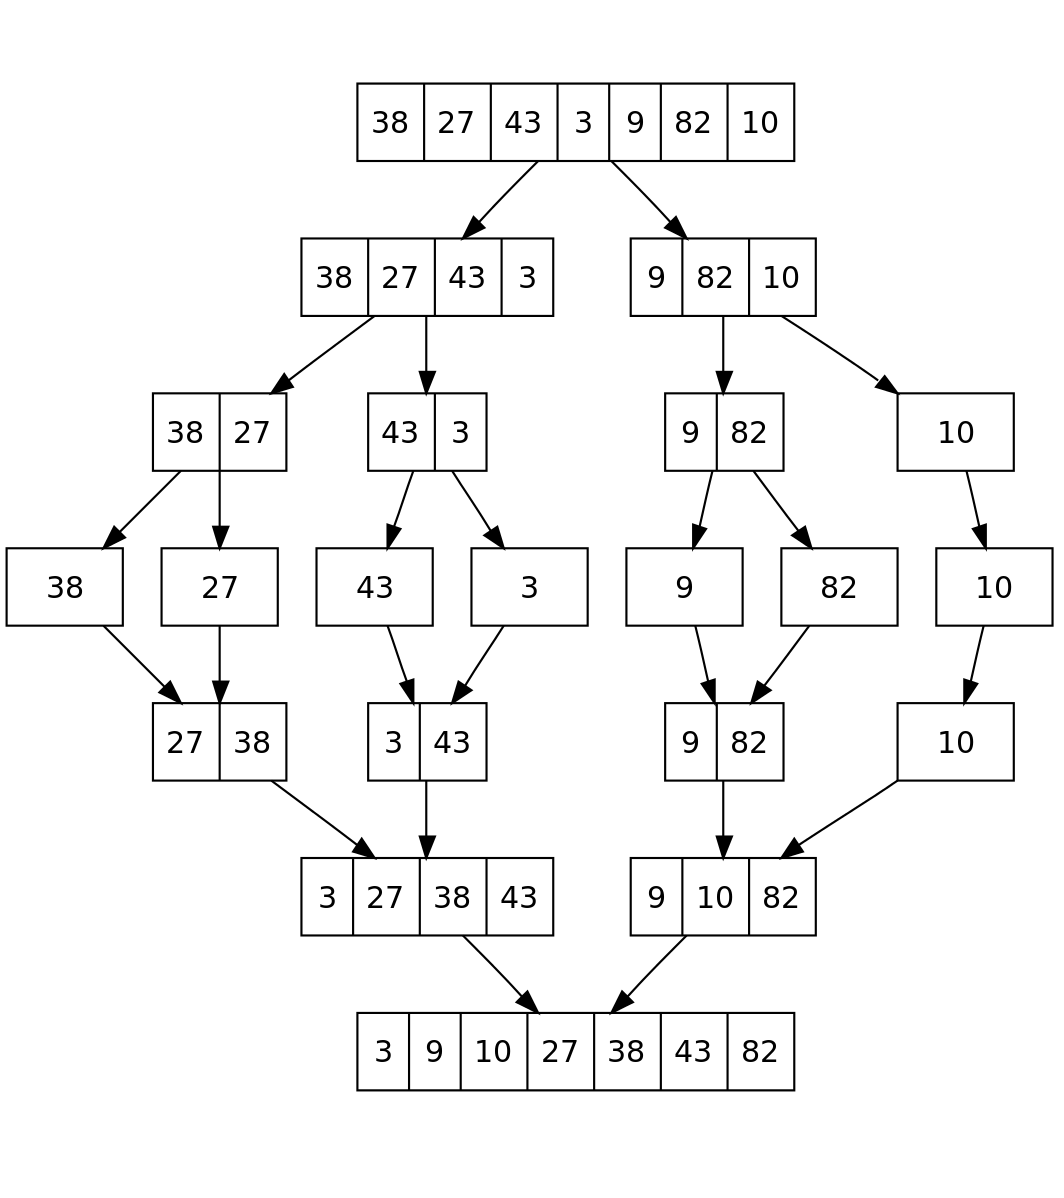
\includegraphics[height=\paperheight]{merge-sort-diagram}}
\begin{frame}[plain]
\end{frame}
}

\begin{frame}
    \vspace{1.5cm}
    \begin{centering}
        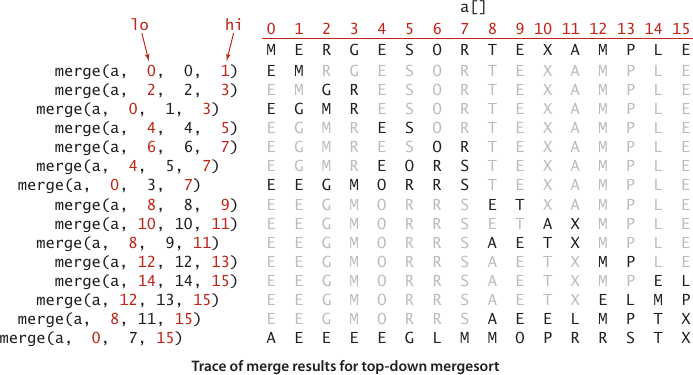
\includegraphics[width=\textwidth]{mergesort-top-down}
    \end{centering}
\end{frame}

\begin{frame}{Trix}
	\begin{itemize}
		\item Notum innsetningarröðun á lítil söfn eða þegar þau eru nær röðuð
		      \begin{itemize}
			      \item Algengt að raunveruleg forritunarmál noti þessa aðferð
			      \item \href{https://docs.oracle.com/javase/8/docs/api/java/util/Arrays.html}{sort} í Java 8
		      \end{itemize}
		\item Neðansækin \eng{bottom-up} sameiningarröðun er meira viðeigandi fyrir eintengda lista
		      \begin{itemize}
			      \item Brjóta vandamálið niður og leysa hlutana endurkvæmt - ofansækin aðferð
			      \item Leysa lítil vandamál sem sameinast í stærri lausn - neðansækin aðferð
		      \end{itemize}
	\end{itemize}
\end{frame}

\begin{frame}
    \vspace{1.5cm}
    \begin{centering}
        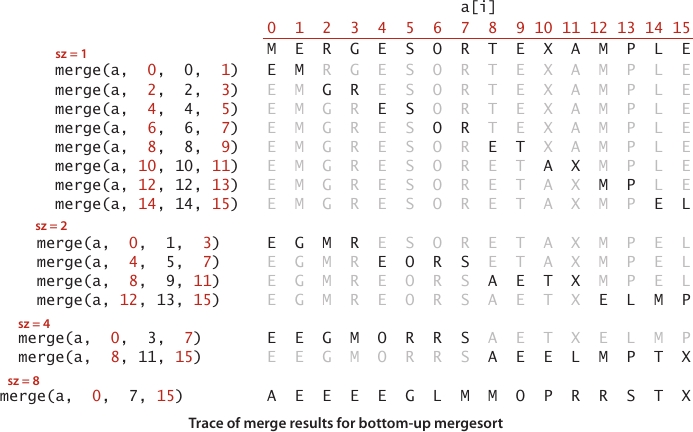
\includegraphics[width=\textwidth]{mergesort-bottom-up}
    \end{centering}
\end{frame}

\begin{frame}{Comparator}
	\begin{columns}
		\column{0.5\textwidth}
		\begin{itemize}
			\item Við getum raðað hlutum sem ekki eru \texttt{Comparable} með því að nota viðeigandi \href{https://docs.oracle.com/javase/8/docs/api/java/util/Comparator.html}{\texttt{Comparator}}
			\item Mikið notað í öðrum málum, munum ekki nota mikið í Java í þessu námskeiði
			      \begin{itemize}
				      \item Gert ráð fyrir þessu í algs4 klösunum
			      \end{itemize}
		\end{itemize}
		\column{0.5\textwidth}
		\begin{center}
			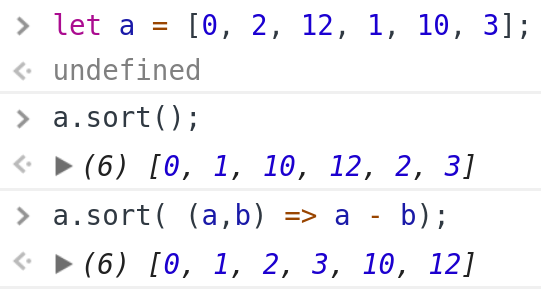
\includegraphics[width=\linewidth]{javascript-comparator}

			Röðun með og án samanburðarfalls í Javascript
		\end{center}
	\end{columns}
\end{frame}

\section{Lokaorð}

\begin{frame}{Tenglar}
	\begin{itemize}
		\item \href{https://www.toptal.com/developers/sorting-algorithms/}{Einföld yfirlitssíða}
		      \begin{itemize}
			      \item Varúð - síðan hefur eitthvað að selja
		      \end{itemize}
		\item \href{https://www.youtube.com/watch?v=kPRA0W1kECg}{The Sound of Sorting}
		      \begin{itemize}
			      \item Varúð - hljóð
		      \end{itemize}
		\item \href{https://www.youtube.com/watch?v=ROalU379l3U}{Röðunardans}
		      \begin{itemize}
			      \item Varúð - dansandi fólk
		      \end{itemize}
		\item \href{https://www.youtube.com/watch?v=es2T6KY45cA}{Vélmenni raða}
	\end{itemize}
\end{frame}

\begin{frame}{Þessi glærupakki}
	Kóða fyrir röðunarreikniritin má finna á \href{http://algs4.cs.princeton.edu/code/}{síðu bókarinnar}. Önnur nafngreind forrit í þessum glærupakka ásamt glærupakkanum sjálfum má finna á \href{https://github.com/Ernir/kennsluefni/tree/master/T2/Code/w6}{Github}.
\end{frame}

\begin{frame}{Næst}
	\begin{itemize}
		\item Miðmisseriskönnun?
		\item Quicksort reikniritið (kafli 2.3), forgangsbiðraðir og hrúgur (kafli 2.4)
	\end{itemize}
\end{frame}


\end{document}
